\documentclass[si.tex]{subfiles}
\begin{document}


Here, we discuss the extent to which models are identifiable when one varies not sensory noise, but rather  stimulus (external) noise.
The model with both sensory and stimulus noise takes the form
\begin{equation}\label{eq:both-noise-types}
    m = F(\theta+\epsilon)+\delta
\end{equation}
where $\epsilon \sim \mathcal{N}(0,\tau^2)$, where $\tau^2$ here denotes the magnitude of stimulus noise.
Whereas sensory noise reflects unavoidable noise of the imperfect neural encoding, stimulus noise is applied to the stimulus. For example, multiple Gabor patches or color patches ma be presented in an array, each with some noise applied to the stimulus value (e.g., \cite{Tomassini2010OrientationUR, Girshick2011CardinalRV, Olkkonen2014TheCT}).
\citet{hahn2024unifying} (Theorem 2) proved that the bias (for positive even $p$) is given as
\begin{equation}\label{eq:stim-noise-bias}
        \underbrace{\left(\frac{1}{\FI(\theta)} + \tau^2\right)    \left( \log p_{prior}(\theta) \right)'}_{Prior\ Attraction}   + \underbrace{\left[ 1               + \frac{p-2}{4}     \frac{1}{1+\tau^2\FI(\theta)}    \right]   \left(\frac{1}{\FI(\theta)}\right)' }_{Likelihood\ Repulsion} + O\left((\sigma^4+\tau^4+\sigma^2\tau^2)\right)
        \end{equation}
        where $\FI$ is the Fisher Information of the sensory encoding, extending the decomposition reviewed in Section~\ref{sec:background}.
        That is, stimulus noise increases attraction, and induces (for $p>2$) a loss-function-dependent reduction of the repulsion.
        While this result is proven for positive even exponents ($p=2,4,6,\dots$), simulations \citet[][SI Appendix, Figure S5]{hahn2024unifying} show that similar behavior holds at other exponents.
        Furthermore,  the variability has the form
        \begin{equation}
            \tau^2 + \frac{1}{\FI(\theta)}  + O\left((\sigma^4+\tau^4+\sigma^2\tau^2)\right)
        \end{equation}
Based on this, in principle, one can identify models by:
\begin{enumerate}
    \item Comparing the variability at two levels of stimulus noise to recover $\frac{1}{\FI(\theta)}$ up to higher-order error.
    \item Then, in the expression for the bias, all except for the green terms are known up to higher-order error:
    \begin{equation}
        \underbrace{\left(\frac{1}{\FI(\theta)} + \tau^2\right)    \textcolor{green}{\left( \log p_{prior}(\theta) \right)'}}_{Prior\ Attraction}   + \underbrace{\left[ 1               + \frac{\textcolor{green}{p}-2}{4}     \frac{1}{1+\tau^2\FI(\theta)}    \right]   \left(\frac{1}{\FI(\theta)}\right)' }_{Likelihood\ Repulsion} + O\left((\sigma^4+\tau^4+\sigma^2\tau^2)\right)
        \end{equation}
        Comparing the bias at two levels of stimulus noise permits identifying these unknowns.
\end{enumerate}
This applies to \emph{all} models, even those in the exceptional set $\Omega$ of our Theorem 2.
Thus, with unbounded amounts of behavioral data, all models are identifiable in principle.

An interesting question is whether varying stimulus noise or sensory noise might be more effective in ensuring identifiability.
Stimulus noise increases the variance:
\begin{equation}
\tau^2 + \frac{1}{\FI(\theta)} + \mathcal{O}(\sigma^4)
\end{equation}
and also increases the prior attraction term.
In contrast, importantly, when $p>2$, stimulus noise \emph{reduces} the loss-function-dependent repulsion, as shown by Equation~\ref{eq:stim-noise-bias}: the higher $\tau^2$ is, the more the likelihood repulsion approaches a loss-function-independent limit
\begin{equation}
\left(\frac{1}{\FI(\theta)}\right)'
\end{equation}
Overall, thus, stimulus noise broadens the response distribution while simultaneously \emph{reducing} the loss-function-dependent repulsion.
This is in contrast to sensory noise, where increasing it leads to an \emph{increase} in the loss-function-dependent repulsion.
We thus expect that adding stimulus noise substantially reduces the signal-to-noise ratio compared to the setting where stimulus noise is zero but sensory noise is varied.

In practice, we indeed find that, at the same number of trials, varying stimulus noise might be less effective in achieving identifiability than sensory noise (Figure~\ref{fig:stim-noise}).




\begin{comment}
python3 evaluateCrossValidationResults_Synthetic_Gardelle_NonF_StimNoise.py SimulateSynthetic_Parameterized_OtherNoiseLevels_Grid_VarySize_WithStimNoise.py_180_2_5_2345_N40000_STEEPPERIODIC_STEEPPERIODIC.txt
python3 evaluateCrossValidationResults_Synthetic_Gardelle_NonF_StimNoise.py SimulateSynthetic_Parameterized_OtherNoiseLevels_Grid_VarySize_WithStimNoise.py_180_8_5_2345_N40000_STEEPPERIODIC_STEEPPERIODIC.txt

python3 RunSynthetic_FreePrior_CosineLoss_OnSim_WithStimNoise_VIZ.py 2 0 10.0 180 SimulateSynthetic_Parameterized_OtherNoiseLevels_Grid_VarySize_WithStimNoise.py_180_2_5_2345_N40000_STEEPPERIODIC_STEEPPERIODIC.txt
python3 RunSynthetic_FreePrior_CosineLoss_OnSim_WithStimNoise_VIZ.py 8 0 10.0 180 SimulateSynthetic_Parameterized_OtherNoiseLevels_Grid_VarySize_WithStimNoise.py_180_8_5_2345_N40000_STEEPPERIODIC_STEEPPERIODIC.txt

python3 CounterfactualModel_VIZ_WithStimNoise.py 2 0 10.0 180 STEEPPERIODIC STEEPPERIODIC 5 2345
python3 CounterfactualModel_VIZ_WithStimNoise.py 8 0 10.0 180 STEEPPERIODIC STEEPPERIODIC 5 2345


\end{comment}


\begin{figure}
\centering

Example 1: $p=2$



\begin{minipage}[c]{0.8\linewidth}
\sideimage{Original}{figures/CounterfactualModel_VIZ_WithStimNoise.py_5_2345_STEEPPERIODIC_STEEPPERIODIC_2_0_10.0_180.pdf}

\sideimage{Fitted}{figures/RunSynthetic_FreePrior_CosineLoss_OnSim_WithStimNoise_VIZ.py_SimulateSynthetic_Parameterized_OtherNoiseLevels_Grid_VarySize_WithStimNoise.py_180_2_5_2345_N40000_STEEPPERIODIC_STEEPPERIODIC.txt_2_0_10.0_180.pdf}
\end{minipage}
\begin{minipage}[c]{0.19\linewidth}
\centering

\ \ \ \ \ \ Negative

\ \ \ \ \ \ Log-Likelihood

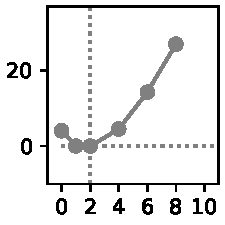
\includegraphics[width=0.98\textwidth]{figures/evaluateCrossValidationResults_Synthetic_Gardelle_NonF_StimNoise.py_SimulateSynthetic_Parameterized_OtherNoiseLevels_Grid_VarySize_WithStimNoise.py_180_2_5_2345_N40000_STEEPPERIODIC_STEEPPERIODIC.txt_RelativeLF.pdf}
\end{minipage}

\ 



Example 2: $p=8$



\begin{minipage}[c]{0.8\linewidth}
\sideimage{Original}{figures/CounterfactualModel_VIZ_WithStimNoise.py_5_2345_STEEPPERIODIC_STEEPPERIODIC_8_0_10.0_180.pdf}

\sideimage{Fitted}{figures/RunSynthetic_FreePrior_CosineLoss_OnSim_WithStimNoise_VIZ.py_SimulateSynthetic_Parameterized_OtherNoiseLevels_Grid_VarySize_WithStimNoise.py_180_8_5_2345_N40000_STEEPPERIODIC_STEEPPERIODIC.txt_8_0_10.0_180.pdf}
\end{minipage}
\begin{minipage}[c]{0.19\linewidth}
\centering

\ \ \ \ \ \ Negative

\ \ \ \ \ \ Log-Likelihood

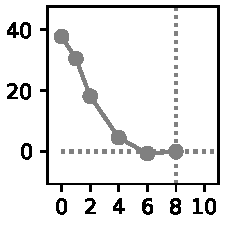
\includegraphics[width=0.98\textwidth]{figures/evaluateCrossValidationResults_Synthetic_Gardelle_NonF_StimNoise.py_SimulateSynthetic_Parameterized_OtherNoiseLevels_Grid_VarySize_WithStimNoise.py_180_8_5_2345_N40000_STEEPPERIODIC_STEEPPERIODIC.txt_RelativeLF.pdf}
\end{minipage}


\caption{Varying stimulus noise, while keeping sensory noise fixed (40K trials).
This can also lead to recoverability, as theoretically demonstrated in Section~\ref{sec:stimulus-noise}.
Comparison to results varying sensory noise (Figures~\ref{fig:recover-model-circ-periodic-periodic} and  \ref{fig:recover-loss-circ-periodic-periodic}) suggests that varying stimulus noise results in a weaker signal then when varying sensory noise; also, the prior at $p=8$ is recovered less successfully then when sensory noise is varied.
Overall, varying stimulus noise can support identifiability, but varying sensory noise is more advisable when feasible.
}\label{fig:stim-noise}

\end{figure}


\end{document}
